\documentclass{article}
\usepackage{graphicx}
\usepackage[utf8]{inputenc}
\graphicspath{ {./img/} }

\title{Appunti di teoria per interviste tecniche}
\author{Marco Savino}
\date{}

\begin{document}

\maketitle

\section{Introduzione}
    Step per entrare in AgileLab:
    \begin{enumerate}
        \item Colloquio conoscitivo HR
        \item Test di conoscenza tecnica
        \item Intervista tecnica
    \end{enumerate}
    
\section{Preparazione al test}
    Il test è diviso in tre macro aree:
    \begin{itemize}
        \item Concetti di software engineering
        \item Database
        \item Sistemi distribuiti (engine)
        \item Machine learning (in minor parte)
    \end{itemize}

\section{Software Engineering}
    \subsection{Programmazione orientata agli oggetti}
        La programmazione orientata agli oggetti è un paradigma di programmazione basato sul concetto di oggetto, ovvero un entità che può contenere dati e operazioni. I dati sono contenuti in campi conosciuti come attributi e le operazioni sono codice scritto in forma di procedure chiamate metodi.
        \paragraph{Classi} Per poter applicare il concetto di oggetto, è necessario prima definirlo: un oggetto viene definito attraverso una classe. La classe serve a stabilire il formato dei dati e le operazioni disponibili dell'oggetto creato tramite essa. Gli oggetti sono quindi delle istanze, ovvero la manifestazione fisica dei dati e delle operazioni descritte all'interno nella classe.
        
        \paragraph{Concetti della Programmazione Orientata agli Oggetti (A. P.I.E.)}
        I concetti alla base di questo paradigma hanno lo scopo di creare metodi e variabili funzionanti, che permettano poi il riutilizzo del codice senza comprometterne la sicurezza.
        
        \paragraph{A - Abstraction (Astrazione)} L'Astrazione è un concetto per il quale si nascondono all'utente i dettagli superflui dell'implementazione, permettendo a questo di concentrarsi sullo sviluppo della logica al di sopra dell'entità astratta fornita, senza doversi preoccupare di come è fatta al suo interno.\\
            \textit{Esempio - Una macchina del caffè rappresenta un'astrazione per l'utente: questo non sa come viene prodotto fisicamente il caffè, ma conosce quanto basta per comandare alla macchinetta di produrne uno. In questo modo, è persino possibile cambiare il meccanismo interno della macchina senza che l'utente ne debba essere a conoscenza.}
        
        \paragraph{P - Polymorphism (Polimorfismo)} Il polimorfismo è un fenomeno in cui una stessa entità assume proprietà differenti a seconda del contesto. In informatica, questo significa poter accedere, in base alla situazione, a diverse classi tramite la stessa interfaccia o a diversi metodi tramite la stesso nome.\\
            In un linguaggio orientato agli oggetti esistono due tipi di polimorfismo:
            \begin{itemize}
                \item \textit{Statico} - All'interno di una stessa classe è possibile definire metodi con lo stesso nome ma con parametri diversi in numero, tipo o ordine: questa proprietà è definita come \textit{overload} del metodo. Al momento dell'invocazione del metodo, verrà eseguito quello selezionato non solo in base al nome, ma anche attraverso le caratteristiche dei parametri della chiamata: si fa così riferimento alla \textit{firma (signature)} del metodo. Si definisce polimorfismo \textit{statico} perché l'associazione fra chiamata e metodo chiamato viene stabilita durante la compilazione.
                \item \textit{Dinamico} - Data una gerarchia di classi, per una sottoclasse è possibile implementare un metodo con la stessa firma di uno della sua superclasse. Alla creazione dell'istanza della sottoclasse, quel metodo avrà la prevalenza su quello corrispondente della superclasse: questa proprietà prende il nome di \textit{overriding}. Inoltre, è possibile che l'istanza di una sottoclasse venga assegnata alla reference della sua superclasse: l'oggetto così appare come una istanza della superclasse ed è possibile invocare solo i metodi di questa. Tuttavia, al momento della creazione dell'istanza della sottoclasse a run-time, alla chiamata del metodo della superclasse viene associato il metodo della sottoclasse. Questa associazione a run-time fra chiamata del metodo e metodo chiamato, selezionando prevalentemente quelli delle sottoclassi, è il fenomeno definito come \textit{late binding} ed è alla base dell'applicazione di costrutti come le \textit{interfacce}.
            \end{itemize}
        
        \paragraph{I - Inherintance (Ereditarietà)} L'ereditarietà è il meccanismo attraverso cui la definizione di una classe deriva da quella di un'altra classe. La prima prende così il nome di sottoclasse e la seconda di super-classe. La sottoclasse condivide lo stesso formato dei dati e le stesse operazioni della sua super-classe, in base alla loro visibilità, e in più ha la possibilità di definirne dei propri a sua volta. Una classe può ereditare una sola altra classe e un numero illimitato di interfacce.
        
        \paragraph{E - Encapsulation (Incapsulamento)} Per definizione, l'incapsulamento consiste nel combinare metodi e attributi in un'unica unità, come ad esempio una classe. Grazie a questo concetto, è possibile nascondere la rappresentazione interna dei dati o il loro stato, rendendoli accessibili solo tramite metodi appositi. Questa tecnica è chiamata \textit{Information Hiding}. Nella pratica, un linguaggio orientato agli oggetti può prevedere principalmente quattro modificatori di visibilità per metodi e attributi:
            \begin{itemize}
                \item \textit{Private} - L'elemento è accessibile solo dalla propria classe e nient'altro.
                \item \textit{Package-private} - Se non si specifica il modificatore di visibilità, l'elemento è accessibile dalla propria classe e da tutte le classi ed eventuali sottoclassi appartenenti allo stesso pacchetto.
                \item \textit{Protected} - L'elemento è accessibile dalla propria classe, dalle classi presenti nello stesso pacchetto e anche dalle sue eventuali sottoclassi presenti in altri pacchetti.
                \item \textit{Public} - L'elemento è accessibile da qualunque classe.
            \end{itemize}
        
    \subsection{S.O.L.I.D.}
        Questo acronimo indica un gruppo di cinque principi da seguire, affinché il codice sia più leggibile e più facile da cambiare in caso di necessità.
        \paragraph{S - Single Resposibilty Principle} \textit{Ogni classe è responsabile di un singolo compito; se cambia il compito, allora cambia anche la classe. Questa deve essere l'unica ragione per cui la classe cambia.}\\
        Esempio: Una classe che si occupa di tenere conto del punteggio di un gioco, non si deve occupare di altro. Questa cambia solo se cambiano le regole del gioco
        \paragraph{O - Open-Closed Principle} \textit{Una classe deve essere aperta all'utilizzo da parte di altre classi, come sua estensione, e chiusa alla possibilità di esser cambiata da altre classi.}\\
        Questo principio si applica attraverso l'Ereditarietà e l'override: creando una sottoclasse ad hoc e sovrascrivendo il metodo di interesse in partenza, si evita di alterare cambiare la classe madre, proprio grazie all'estensione della stessa.
        \paragraph{L - Liskov Substitution Principle} \textit{Una proprietà dell'oggetto X di una classe T deve essere valida anche per un oggetto Y di classe S, dove S è sottoclasse di T.}\\
        Questo implica che, in un programma, le istanze di una classe dovrebbero essere sempre sostituibili dalle istanze di una sua sottoclasse. A livello pratico, ogni suo metodo deve poter accettare gli argomenti del corrispettivo metodo della classe madre e ritornare lo stesso tipo di valore. In alcuni casi però, questo ha dei limiti: una classe Rettangolo crea un'istanza grazie agli argomenti base e altezza, ma una sua sottoclasse Quadrato utilizzerebbe come argomento solo il lato; in questo caso, per rispettare il principio la classe Quadrato non deve essere sottoclasse di Rettangolo.
        \paragraph{I - Interface Segregation Principle}
            \textit{"Un cliente non dovrebbe essere costret-to a dipendere da una interfaccia che non usa" - Robert C. Martin}\\
            Non bisogna aggiungere funzionalità che non vengono utilizzate a una interfaccia. Questo perché, aggiornando l'interfaccia, bisogna aggiornare anche tutto ciò che ne dipende. L'ideale è quindi creare un'interfaccia a parte che non abbia influenze su quella di partenza.
        \paragraph{D - Dependency Inversion Principle} 
            \textit{Moduli di altro livello non devono dipendere da moduli di basso livello, ed entrambi devono basarsi su astrazioni; le astrazioni non devono dipendere dai dettagli, ma i dettagli dalle astrazioni.}\\
            Si dà importanza al disaccoppiamento fra moduli: l'implementazione di questi potrà cambiare senza influire sulla loro comunicazione. A livello pratico, si applica la cosiddetta \textit{Dependency Injection}.

    \subsection{Sviluppo software}
        \paragraph{Ciclo di vita del software} il \textit{Software Development Life Cycle} viene definito con 6 fasi:
            \begin{enumerate}
                \item \textit{Raccolta dei requisiti}: "Qual è il problema attuale?"
                \item \textit{Pianificazione}: "Che cosa vogliamo?"
                \item \textit{Progettazione}: "Come otteniamo quello che vogliamo?"
                \item \textit{Implementazione}: "Creiamo quello che vogliamo"
                \item \textit{Test e integrazione}: "Abbiamo ottenuto quello che volevamo? Funziona?"
                \item \textit{Manutenzione}: "Miglioriamo quello che abbiamo ottenuto"
            \end{enumerate}
            Queste fasi possono essere gestite in numerosi modi diversi, definiti come modelli:
            \begin{itemize}
                \item \textit{Modello a cascata}: le fasi vengono svolte linearmente una dopo l'altra.
                \item \textit{Modello a V}: estensione del modello a cascata, testando però dopo ogni fase.
                \item \textit{Modello iterativo}: si crea una versione base che viene migliorata tramite frequenti aggiornamenti uno dopo l'altro.
                \item \textit{Modello agile}: il prodotto è gestito a cicli e con frequenti aggiornamenti, per  migliorare in base al feedback dell'utente.
                \item \textit{Modello a spirale}: Estensione del modello iterativo, vengono ripetute tutte le fasi del SDLC
                \item \textit{Big Bang Model}: Viene lasciato tutto in mano a sviluppatori esperti, che si concentrano da subito sull'implementazione
            \end{itemize}
        \paragraph{Testing} Ci sono diversi tipi di test, che servono a garantire il  corretto funzionamento del dofice in tutte le occasioni:
            \begin{itemize}
                    \item \textit{Analisi statica}: esamina tutti i possibili comportamenti del codice che potrebbero manifestarsi a run-time. Include sempre la revisione del codice, l'ispezione del codice, l'analisi algoritmica e la prova di correttezza.
                    \item \textit{Analisi dinamica}: coinvolge l'esecuzione del codice per esporre errori e malfunzionamenti.
                    \item \textit{Black box}: si testa il codice attraverso input e output, ignorando il modo in cui è implementato il codice.
                    \item \textit{White box}: presupponendo la conoscenza dell'implementazione, si effettuano i test concentrandosi sulla struttura del codice e sulla logica di business (vedi \textit{statement coverage, branch coverage, path coverage}). 
                    \item \textit{Scripted box}: specifico test basato su una serie di step prefissati pensato per validare un preciso requisito.
                    \item \textit{Exploratory}: il tester simula il comportamento dell'utente finale e si basa sull'intuito per rilevare problemi nascosti o non previsti in precedenza.
                    \item \textit{Manual}: viene eseguito da persone.
                    \item \textit{Automated}: viene eseguito da software automatizzati.
                \end{itemize}

    \subsection{Design Pattern}
        \subsubsection{Pattern Creazionali}
            I pattern creazionali forniscono diversi meccanismi per la creazione degli oggetti, puntando a migliorare la flessibilità e il riutilizzo del codice.
            \paragraph{Factory} Viene applicato per disaccoppiare il codice di costruzione dell'oggetto dal codice in cui viene utilizzato quell'oggetto, seguendo il Single Resposibilty Principle e Open-Closed Principle.
                I passi per impostare il pattern Factory sono i seguenti:
                \begin{enumerate}
                    \item Si definisce un'interfaccia a partire dagli oggetti da istanziare
                    \item Si crea una classe astratta contenente un metodo astratto che restituisce il tipo dell'interfaccia degli oggetti
                    \item Si creano tante classi "fabbrica" quanti sono gli oggetti in questione e ognuna di queste erediterà la classe astratta
                    \item Ogni classe "fabbrica" implementa il metodo astratto per restituire una istanza dello specifico oggetto per cui la classe è stata creata
                    \item Per creare un oggetto in particolare, invece di invocarne il costruttore, verrà chiamato il metodo della sua classe "fabbrica" che ne restituirà uno. 
                \end{enumerate}
                \textit{Esempio - Esistono le classi Auto e Moto: queste possono essere implementazioni di una nuova o già esistente interfaccia Veicolo.
                    Si crea quindi una classe astratta FabbricaVeicolo che conterrà il metodo astratto creaVeicolo().
                    Questa classe viene ereditata da due sottoclassi, FabbricaAuto e FabbricaMoto, nelle quali il metodo creaVeicolo() restituirà rispettivamente una istanza di Auto e una di Moto, entrambe di tipo Veicolo.
                    Infine, si inizializza una istanza di FabbricaVeicolo come FabbricaAuto o FabbricaMoto, in base alle necessità.
                    In questo modo, è possibile passare a chi lo richiede l'istanza di tipo FabbricaVeicolo in modo del tutto indipendente da ciò che contiene, e potrà utilizzarne il metodo creaVeicolo() per ottenere un'istanza definita a run-time.
                }
            \paragraph{Abstract Factory} Il concetto di base è lo stesso del pattern Factory, ma con la differenza che le classi da istanziare sono classi "fabbrica".
                I passi da seguire per implementare il pattern sono i seguenti:
                \begin{enumerate}
                    \item Definire una interfaccia per ogni categoria di oggetti che le classi "fabbrica" si occuperanno di creare
                    \item Creare una interfaccia per le classi "fabbrica" con i metodi astratti di creazione degli oggetti, ciascuno del tipo astratto prima definito
                    \item Implementare le classi "fabbrica" con l'interfaccia definita, implementando i metodi astratti secondo la tipologia effettiva di oggetto corrispondente alla classe stessa
                    \item Creare una istanza della classe "fabbrica" scelta
                    \item Per creare un oggetto specifico, sarà sufficiente invocare il metodo apposito, la cui chiamata sarà indipendente dal tipo di classe "fabbrica" e dall'oggetto scelto
                \end{enumerate}
                \textit{Esempio - Vi è la necessità di creare entità come pulsanti o checkbox in base allo stile del sistema operativo presente.
                    Si definisce quindi una interfaccia i pulsanti, una per le checkbox e in generale una per ogni entità simile.
                    Si crea poi una interfaccia per le classi "fabbrica", contentente i metodi astratti per la creazione delle entità, del tipo della rispettiva interfaccia.
                    Si implementano quindi diverse classi "fabbrica", una per ogni sistema operativo previsto, le quali implementeranno i metodi astratti con il tipo specifico delle diverse entità.
                    Infine, sarà sufficente fornire una istanza della classe "fabbrica" scelta per permettere di creare le istanze delle entità richieste secondo uno stile uniforme.
                }
            \paragraph{Builder} Permette di costruire oggetti complessi procedendo step by step.
                Il concetto alla base è quello di racchiudere in una classe "Builder" tutti i passi necessari per la costruzione di un oggetto, invece che dover specificare tutto nel costruttore fin da subito o aver diverse classi per ogni sua possibile variante.
                La classe builder contiene quindi una istanza dell'oggetto, un metodo Get dedicato e tutti i metodi richiesti per la parametrizzazione dell'oggetto.
                Tuttavia, vi possono anche essere altri modi per costruire oggetti diversi fra loro: si defnisce quindi una interfaccia che racchiude tutte le classi builder, che implementeranno i metodi astratti in base al loro specifico oggetto.
                Infine, per astrarsi dalla logica dei diversi builder e per stabilire un ordine dei passi da effetuare, si definisce una classe "Director" che li gestisce, nascondendone l'implementazione all'utente.\\
                \textit{Esempio - Partendo da due classi AutoCambioAutomatico e AutoCambioManuale, si definisce una interfaccia per le loro due classi Builder: queste classi saranno idendiche in tutto tranne che nella costruzione del cambio.
                    Nel frattempo, si definisce anche una classe Director, la quale avrà diversi metodi preimpostati per la costruzione di auto come berline, SUV o spider.
                    Si inizializza quindi una istanza della classe builder, in base alla selezione del cambio automatico o manuale.
                    Si istanzia infine la classe director e si invoca il metodo in base alla tipologia di auto scelta, e gli si passa il builder instanziato per specificare al director come costruire l'auto.
                }
            \paragraph{Singleton} Assicura che venga creata una sola istanza di una certa classe, che viene resa accessibile globalmente.
                Durante l'implementazione della classe, il costruttore viene reso privato.
                Affinché quindi la classe sia utilizzabile, viene definito un metodo statico pubblico e un attributo statico privato del tipo della classe stessa.
                Quando il metodo pubblico viene invocato per la prima volta, l'attributo risulta nullo: si procede quindi alla sua inizializzazione e alla restituzione al chiamante.
                Se il metodo viene chiamato successivamente, questo si accorgerà che l'istanza esiste già, perciò la ritornerà direttamente, senza crearne una nuova.\\
                \textit{Esempio - Nel momento in cui bisogan aprire una connessione ad un database, è utile che questa venga istanziata una sola volta, per poi continuare a riferirsi ad essa.
                    Se il metodo statico pubblico GetConnection() viene chiamato per la prima volta e l'attributo Database risulta nullo, si procede ad aprire la connessione per poi ritornarla.
                    Altrimenti, viene restituito direttamente l'attributo Database, già istanziato.
                }  
            \paragraph{Prototype} Permette di creare una \textit{deep copy} di oggetti esistenti senza rendere il codice dipendente dalla loro classe.
                Dipende molto dal linguaggio di programmazione, ma l'idea generale è quella di avere un metodo dedicato che crei una nuova istanza della classe copiandone i paramentri, imposto anche tramite una interfaccia spesso nominata "Clonable".
                Risulta importante rispetto alla creazione di una \textit{shallow copy} perché permette di modificarne i parametri senza influenzare l'oggetto originale. 
        
        \subsubsection{Pattern Strutturali}
            \paragraph{Adapter} Permette a oggetti con diverse interfacce di comunicare.
                Si realizza attraverso una classe Adapter che eredita la interfaccia richiesta dal client e continene al suo interno una istanza del Service.
                Inoltre, al suo interno viene implementato tutto il necessario per rendere compatibili le comunicazioni fra client e service.
                \textit{Esempio - Un provider di dati stock fornisce i dati in formato XML, ma le librerie per analizzare tali dati accettano solo il formato JSON.
                    Si implementa quindi una classe che implementa l'interfaccia del provider, in grado di richiedere i dati.
                    Nella stessa classe si utilizza un metodo per poter convertire i dati da XML a JSON, in modo tale da poter utilizzare le istanze delle librerie correttamente.
                }
            \paragraph{}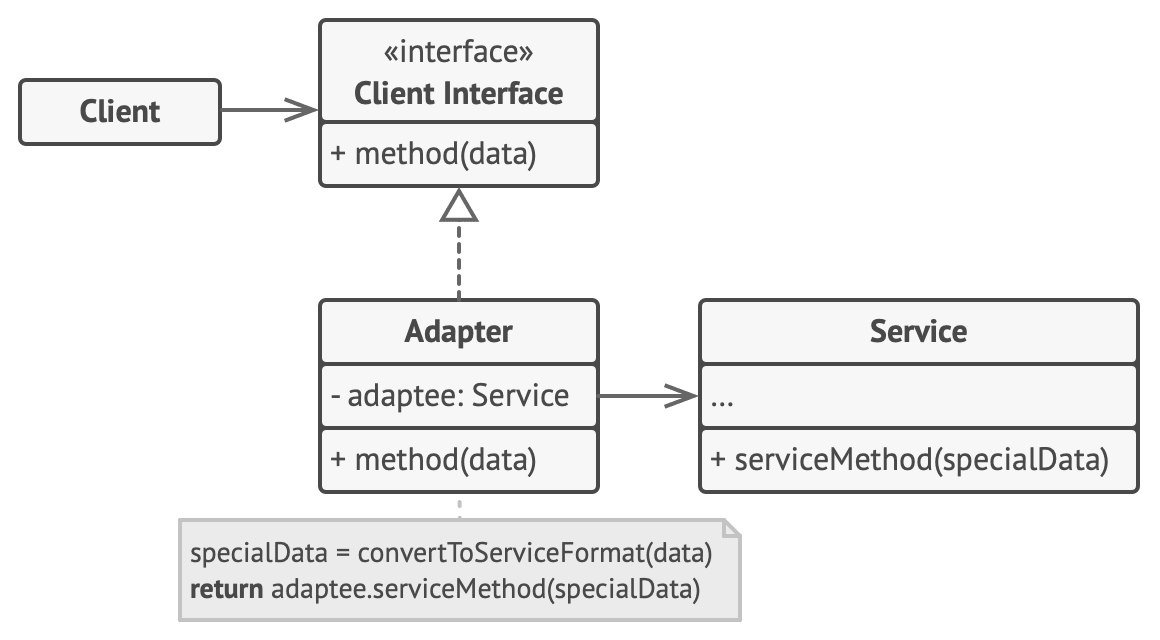
\includegraphics[scale=0.25]{./img/adapter.png}

            \paragraph{Bridge} Punta a suddividere classi complesse o un insieme di classi fortemente correlate in due gerarchie di classi, dette \textit{astrazione} e \textit{implementazione}, indipendenti tra loro.\\
                \textit{Esempio - Allo stato attuale, esistono la classe TelecomandoTV correlata alla classe TV e la classe TelecomandoStereo correlata alla classe Stereo.
                    Applicando il pattern Bridge, si pensa ad una classe Telecomando come \textit{astrazione} ed a una interfaccia Dispositivo come \textit{implementazione}, predisposte con metodi correlati e prestabiliti.
                    In questo modo, la classe Telecomando sostituisce le due classi distinte TelecomandoTV e TelecomandoStereo e, in caso di necessità, può essere ereditata ed espansa con ulteriori funzionalità.
                    Questa classe ha inoltre una istanza di Dispositivo, interfaccia a sua volta implementata da TV e Stereo.
                    In questo modo, è possibile modificare Telecomando o le classi concrete come TV e Stereo in modo del tutto indipendente le une dalle altre.
                }
            \paragraph{}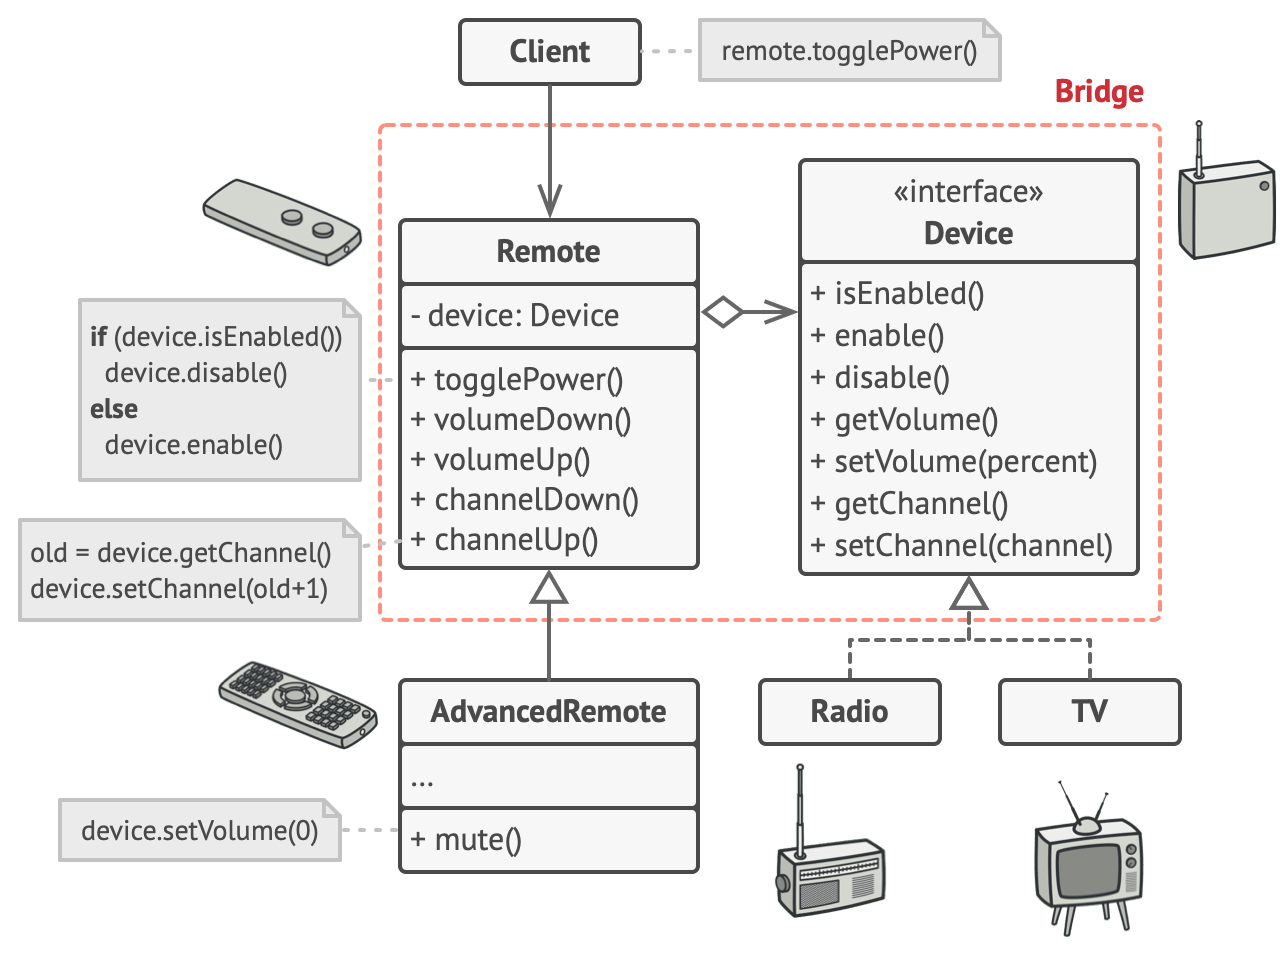
\includegraphics[scale=0.25]{./img/bridge.png}
                
            \paragraph{Composite} Permette di organizzare gli oggetti in strutture ad albero, per poi trattarli come una unica entità.
                Si crea una interfaccia che viene implementata sia dalle \textit{foglie} appartententi al albero che dai \textit{rami}.
                In questo modo, un ramo può contenere una lista di istanze del tipo dell'interfaccia, a prescindere che siano foglie o altri rami.             
            \paragraph{}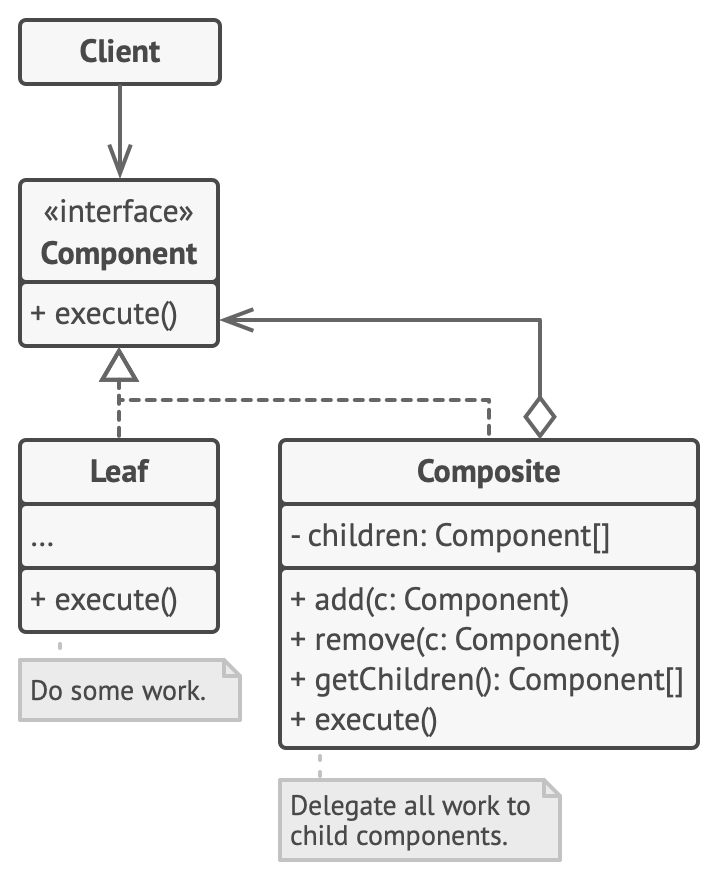
\includegraphics[scale=0.25]{./img/composite.png}
            
            \paragraph{Decorator} Permette di aggiungere nuove funzionalità agli oggetti inserendoli dentro degli oggetti \textit{wrapper}, che contengono le funzionalità richieste.
            \paragraph{}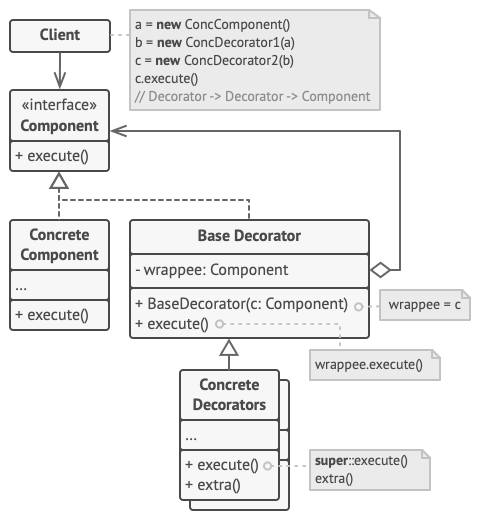
\includegraphics[scale=0.5]{./img/decorator.png}

            \paragraph{Facade} Fornisce una interfaccia semplificata per utilizzare un qualsiasi isnieme complesso di classi.
            \paragraph{}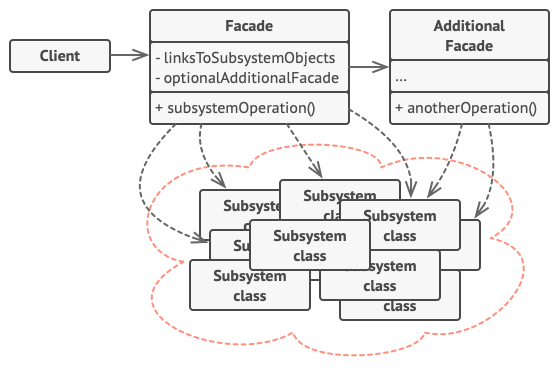
\includegraphics[scale=0.5]{./img/facade.png}

            \paragraph{Flyweight} Aiuta a ottimizzare l'utilizzo di RAM grazie alla condivisioni di elementi comuni fra diversi oggetti invece che tenerli separati e ripetuti oggetto per oggetto.
            \paragraph{}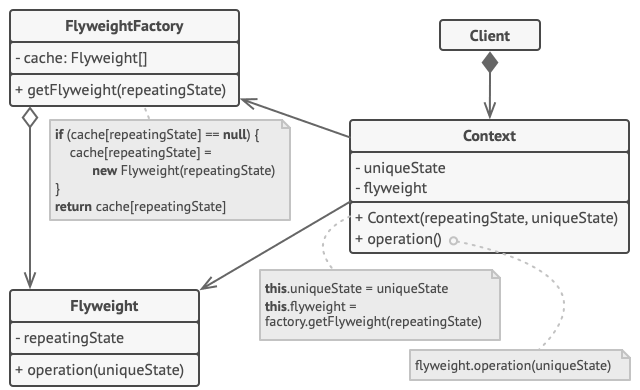
\includegraphics[scale=0.5]{./img/flyweight.png}

            \paragraph{Proxy} Fornisce un sostituto detto \textit{proxy} per un altro oggetto.
                Un proxy gestisce l'accesso all'oggetto originale, permettendo quindi di gestire le richieste.
            \paragraph{}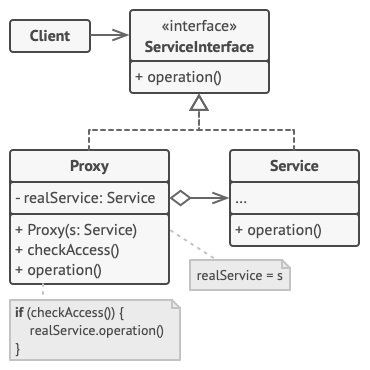
\includegraphics[scale=0.6]{./img/proxy.png}
                
        \subsubsection{Pattern Comportamentali}
        
            \paragraph{Chain of Resposibilty}
            \paragraph{Command}
            \paragraph{Iterator}
            \paragraph{Mediator}
            \paragraph{Memento}
            \paragraph{Observer}
            \paragraph{State}
            \paragraph{Strategy}
            \paragraph{Template Method}
                
    \subsection{Strutture dati}
        \paragraph{Binary Tree}
    
    \subsection{Altri concetti}
        \paragraph{Dependency Injection} A partire da un'interfaccia, che ha un livello di astrazione più alto di una classe, si applica la dipendenza, ovvero la classe che la implementa. La dipendenza può cambiare senza che l'interfaccia ne risenta, persino a run-time. In questo caso, si parla di \textbf{Binding Dinamico}.
        \paragraph{Inversion of Control} Principio di programmazione secondo cui il controllo del flusso dello sviluppo di una applicazione viene lasciato alla piattaforma che si utilizza, la quale prende il nome di \textbf{framework}. I vantaggi pirncipali consistono nel riutilizzo del codice e nel permettere all'utente di concentrarsi sull'implementazione dei moduli, piuttosto che sulla loro comunicazione. La Dependency Injection è un modo di implementare il principio di Inversion of Control.

\section{Database}
    \subsection{A.C.I.D.}
        Proprietà che devono avere delle transazioni in un database.
        \paragraph{A - Atomic} Una transazione deve essere un'unità "atomica", ovvero non può essere suddivisa in più parti e, una volta iniziate, deve essere portata a termine.
        \paragraph{C - Consistency} La transazione deve rispettare i vincoli di integrità del database.
        \paragraph{I - Isolation} Una transazione deve essere eseguita in modo isolato e indipendente dalle altre.
        \paragraph{D - Durability} Definibile anche come \textit{persistenza}, implica che, una volta che la transazione abbia effettuato una \textit{commit}, i cambiamenti apportati devono essere conservati. 
    
    \subsection{Relazioni}
        \paragraph{Uno a uno} A un record di una tabella, corrisponde uno e un solo record di un'altra tabella. Si realizza ponendo il vincolo UNIQUE sulla foreign key.
        \paragraph{Uno a molti} A un record di una tabella corrispondono uno o più record di un'altra tabella. Si realizza ponendo il vincolo della foreign key.
        \paragraph{Molti a molti} A più record di una tabella possono corrispondere più record di un'altra tabella. Per realizzarlo fra due tabelle è necessario introdurre una terza tabella intermedia che leghi la foreign key della prima con la primary key della seconda.
    
    \subsection{Normalizzazioni}
        \paragraph{Forma zero} La tabella dispone di chiave primaria.
        \paragraph{Prima forma normale} La tabella presenta campi atomici, senza tabelle al loro interno. Facendo riferimento al modello E-R, significa che eventuali attributi composti sono stati trasformati in entità, cioè tabelle, a loro volta.
        \paragraph{Seconda forma normale} In caso la chiave primaria sia composta da più campi, ogni altro campo del record deve essere \textit{funzionalmente dipendente} da essa nella sua sua interezza, e non solo da alcune sue parti.
        \paragraph{Terza forma normale} Ogni campo di un record deve essere funzionalmente dipendente solo e soltato dalla chiave primaria, in modo diretto.
        \paragraph{Forma normale di Boyce e Codd} Formulazione leggermente più forte della terza forma normale: ogni campo deve essere funzionalmente dipendente da una super-chiave.
    
    \subsection{Costraints}
        I vincoli sono delle regole che vengono assegnate per garantire l'accuratezza e l'affidabilità di una tabella. Possono essere \textit{column level} oppure \textit{table level}. I vincoli più comuni in SQL sono:
        \begin{itemize}
            \item \textit{NOT NULL}: il campo della colonna non può avere valore NULL.
            \item \textit{UNIQUE}: nella colonna non può esserci lo stesso valore più volte.
            \item \textit{PRIMARY KEY}: unione dei vincoli NOT NULL e UNIQUE, ve ne è solo uno per tabella.
            \item \textit{FOREIGN KEY}: associa i valori della colonna a quelli della chiave primaria di un'altra tabella; impedisce la cancellazione della tabella grazie a questo collegamento, se non specificato diversamente. Conosciuto anche come \textit{vincolo di integrità referenziale}.
            \item \textit{CHECK}: si assicura che i valori in una colonna soddisfino specifiche condizioni.
            \item \textit{DEFAULT}: assegna un valore di default se il campo non viene valorizzato.
            \item \textit{CREATE INDEX}: puntatore alla cella che permette il rapido accesso ai dati.
        \end{itemize}
    
    \subsection{Big Data - Le cinque V}
    
    \subsection{Altri concetti}
        \paragraph{Dipendenza funzionale} In un record di una tabella, un campo è funzionalmente dipendente da un altro campo quando, in presenza di un determinato valore del primo, si ottiene un determinato valore del secondo.
        \paragraph{NoSQL}

\section{Sistemi distribuiti}
    Un sistema distribuito è un insieme di componenti che comunicano e coordinano le loro azioni attraverso lo scambio di messaggi.
    \subsection{Caratteristiche dei sistemi distribuiti}
        \paragraph{Vantaggi}
            \begin{itemize}
                \item \textit{Scalabilità} - Il sistema è scalabile orizzontalmente attraverso l'impiego di un numero potenzialmente illimitato di macchine economiche.
                \item \textit{Affidabilità} - Se un componente cessa di funzionare, il resto del sistema può continuare a operare, anche se a regime ridotto.
                \item \textit{Prestazioni} - Le applicazioni su sistemi distribuiti tendono a suddividere problemi complessi in numerosi parti più semplici, la cui elaborazione viene parallelizzata su più macchine.
            \end{itemize}
        \paragraph{Svantaggi}
            \begin{itemize}
                \item \textit{Coerenza o disponibilità} - Poiché i sistemi distribuiti offrono per definizione piena \textit{partition tollerance (tolleranza delle partizioni)}, bisogna scegliere 
            \end{itemize}
        
    \subsection{Hadoop}

\section{Fonti}
    \paragraph{Wikipedia}
    \paragraph{Stackify}
        \begin{itemize}
            \item https://stackify.com/oops-concepts-in-java/
            \item https://www.baeldung.com/cs/distributed-systems-guide
        \end{itemize} 
    \paragraph{EnjoyAlgorithms}
    \paragraph{Baeldung}
    \paragraph{Refactoring Guru}
            
            
            

\end{document}
